\documentclass[11pt,a4paper]{article}
\usepackage[margin=25mm]{geometry}
\usepackage[T1]{fontenc}
\usepackage[utf8]{inputenc}
\usepackage{lmodern,microtype}
\usepackage{amsmath,amssymb}
\usepackage{graphicx,booktabs,tabularx,array,longtable}
\usepackage{float,placeins}
\usepackage[font=small,labelfont=bf]{caption}
\usepackage[hidelinks]{hyperref}
\usepackage{xcolor}
\usepackage{enumitem}
\setlength{\parindent}{0pt}
\setlength{\parskip}{5pt}
\setlist{nosep,leftmargin=*}
\renewcommand{\topfraction}{0.9}
\renewcommand{\bottomfraction}{0.85}
\renewcommand{\textfraction}{0.1}
\renewcommand{\floatpagefraction}{0.9}
\newcommand{\todo}[1]{\textcolor{red}{\textbf{[To be completed: #1]}}}
\newcommand{\eps}{\varepsilon}
\begin{document}
\begin{center}
{\LARGE\bfseries Visualizing Explainable Density-Based Clustering\par}
\vspace{4pt}
{\large A Study of DBSCAN and ExDBSCAN\par}
\end{center}
\begin{abstract}
DBSCAN identifies clusters of arbitrary shape and labels isolated observations as noise, but a cluster plot alone does not explain an individual assignment. We implement DBSCAN and the ExDBSCAN counterfactual procedure, and provide visual views of the overall clustering, a selected point's neighborhood, and a possible change in assignment. Controlled synthetic datasets and a snapshot of 1,260 Southern California earthquake locations are used to examine correctness, parameter sensitivity, and counterfactual feasibility. In the saved experiments, the greedy method returned 3,184 counterfactuals, all of which passed an independent target-neighborhood check. With one feature fixed, however, some requests had only partial results or no feasible result. The examples illustrate how explanations depend on the clustering parameters and on the constraints placed on a point.
\end{abstract}

\section{Introduction}
Clustering organizes unlabelled observations into groups that reflect their relationships. DBSCAN forms groups from dense neighborhoods instead of requiring a fixed number of clusters. It can identify curved or irregular groups and mark sparse observations as noise \cite{ester1996}. These properties make it a useful method for spatial event data, where clusters may have complex shapes and some events may be isolated.

A plot of the final labels gives a useful overview, but does not by itself explain why a particular point is a core point, a border point, or noise. It also does not answer a related question: what change would place that point within reach of another cluster? ExDBSCAN addresses the second question with counterfactual explanations based on the density structure of a fitted DBSCAN model \cite{matthews2026}.

This project combines the two methods with visual explanations. The global view presents the clustering; the local view exposes the neighborhood that determines a point's role; and the counterfactual view compares the original point with an alternative location. We evaluate these views and the underlying algorithms on controlled examples and a real spatial dataset. The experiments also examine how parameters and fixed features affect the explanations.
Figure~\ref{fig:local} shows a small case that can be checked manually. With $\eps=0.81$ and MinPts $=3$, point 0 has only two points in its own neighborhood, including itself, but lies within the neighborhood of core point 3. It is therefore a border point. Point 4 has no neighboring core point and is noise.
\begin{figure}[htbp]
\centering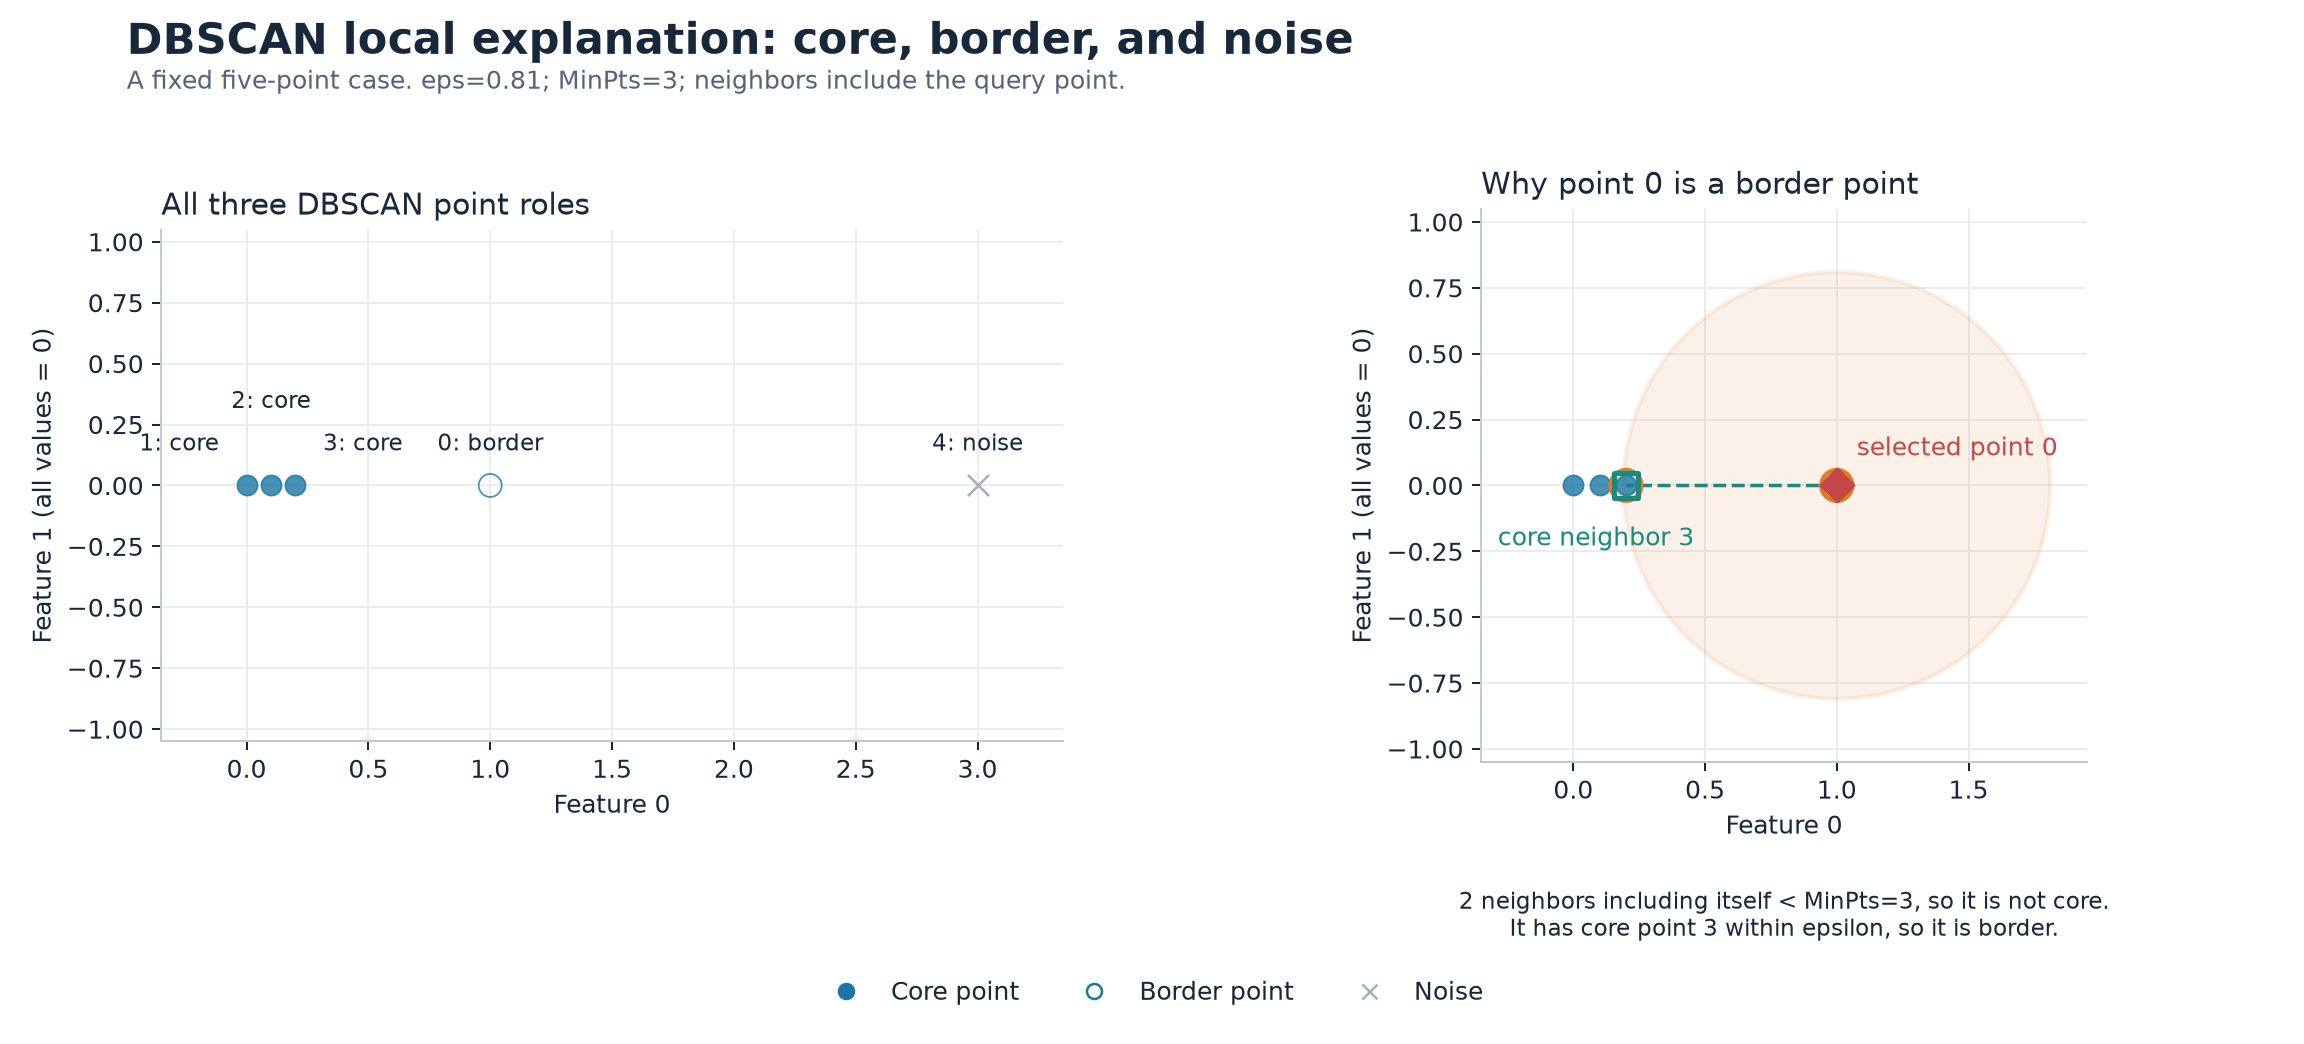
\includegraphics[width=\linewidth,height=0.29\textheight,keepaspectratio]{images/01a_dbscan_explanation.png}
\caption{A five-point local example of core, border, and noise roles. The selected point is border because it is reachable from a core point, although it is not core itself.}
\label{fig:local}
\end{figure}
\section{Background}
\subsection{Density-based clustering}
For a point $p$, its $\eps$-neighborhood $N_{\eps}(p)$ contains all observations at distance at most $\eps$ from $p$, including $p$ itself. A point is \emph{core} if its neighborhood contains at least MinPts observations. A non-core point within the neighborhood of a core point is a \emph{border} point; a point that is neither core nor border is \emph{noise}. DBSCAN expands clusters through chains of neighboring core points and attaches border points to them \cite{ester1996}.

Both parameters affect the result \cite{schubert2017}. A small $\eps$ can split a sparse group into several clusters or noise, while a large $\eps$ can connect separate groups. A larger MinPts requires greater local density. Border points can be adjacent to core points from more than one cluster; an implementation must therefore use a consistent assignment rule.

\subsection{Counterfactual explanations}
A counterfactual describes a change from a query point $p$ to a point $p'$ that satisfies a desired condition. In this study the condition is that $p'$ lies in the $\eps$-neighborhood of a core point belonging to a target cluster. The direction and size of $p'-p$ make the change inspectable. With several explanations, proximity to the original point and diversity among the alternatives are both relevant. Mothilal et al.\ \cite{mothilal2020} discuss diversity and feasibility for counterfactual explanations of classifiers. For clustering, Spagnol et al.\ \cite{spagnol2024} use spatial information to guide counterfactual search. FACE \cite{poyiadzi2020} also considers the feasibility of paths between the original and alternative instances; the straight arrows in our visualizations indicate feature changes, rather than feasible routes.

ExDBSCAN uses a weighted graph of core points to reflect density connectivity when selecting reference points \cite{matthews2026}. A graph path can be longer than the straight-line distance and thus capture the shape of a curved cluster. The explanations in this report are defined with respect to a fitted clustering: entering a target core neighborhood does not necessarily imply a unique label after the data are changed and DBSCAN is fitted again.

\subsection{Visual analysis of clustering}
Visual analytics can help users compare clustering results and inspect individual groups. For example, Clustervision combines coordinated views with measures for exploring different clusterings \cite{kwon2018}. Our interface focuses on the local density relationships and counterfactual changes for a selected DBSCAN result.

\section{Methods and Implementation}
\subsection{DBSCAN}
The implementation takes a finite numeric dataset, a positive radius $\eps$, and MinPts. It computes Euclidean neighborhoods using the closed condition $\|p-q\|\leq\eps$, determines the point roles, and expands each cluster with a queue. A non-core point can be attached to a cluster but does not expand it. Duplicate observations are retained in neighborhood counts. If a border point is reachable from more than one cluster, it is assigned to the first discovered cluster. The implementation does not automatically standardize features, so the distance units and feature preparation must be chosen for the dataset.



\subsection{ExDBSCAN reference selection}
Following ExDBSCAN's core-point graph and greedy selection approach \cite{matthews2026,matthews2026supp}, we identify candidate core points in the target cluster after fitting DBSCAN. Candidate points belonging to the same cluster are connected when their distance is at most $\eps$; edges are weighted by Euclidean distance. Dijkstra's algorithm computes graph distances used by the selection procedure. Candidate reference points are selected greedily using an energy that combines attraction to the query and a penalty for choosing references that are close in the graph:
\begin{equation}
E(S)=\sum_{q\in S}\|p-q\|^2+\sum_{i<j}\frac{1}{\widehat{D}_G(q_i,q_j)}.
\end{equation}
Here $S$ is the selected set and $\widehat{D}_G$ is the scaled graph distance. Disconnected pairs have zero reciprocal penalty. The implementation uses the mean positive weight of distinct undirected graph edges in its scaling; this is an explicit interpretation of the normalization described in the paper.

For each selected reference $q$, an unconstrained query outside its neighborhood is projected toward the closest point on the $\eps$-ball around $q$. The result is then checked independently against the fitted target core points. Figure~\ref{fig:ex} shows a curved cluster: the illustrated graph path between two references is about 3.11 units, compared with a straight-line distance of about 2.00. The resulting alternatives illustrate how reference selection can spread explanations along the cluster. Greedy selection does not guarantee a global optimum for multiple explanations.
\begin{figure}[htbp]
\centering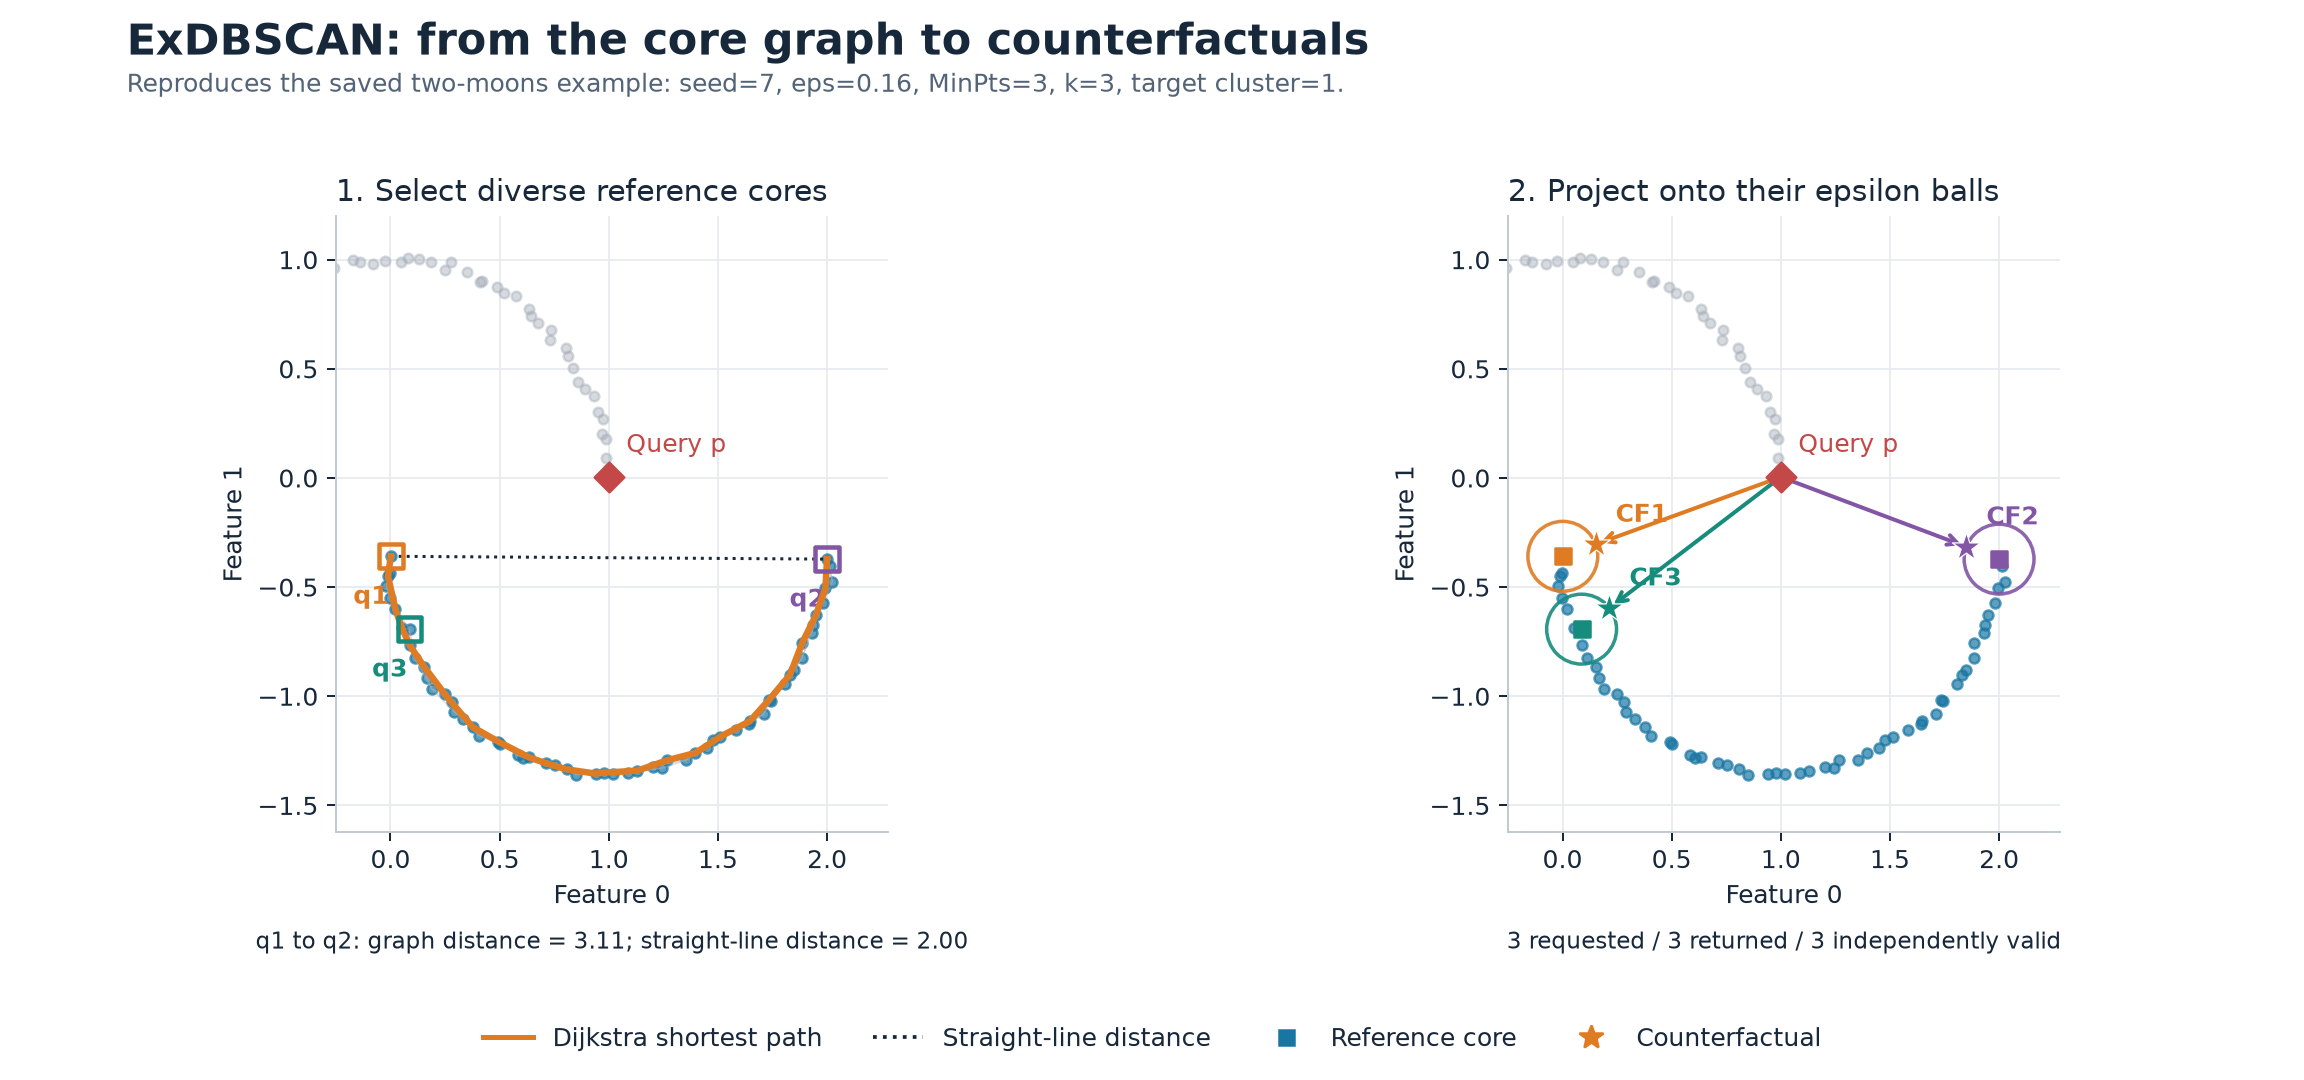
\includegraphics[width=\linewidth,height=0.30\textheight,keepaspectratio]{images/02_exdbscan.png}
\caption{Core-point graph, selected references, and counterfactuals in a synthetic example. Arrows show feature changes, not travel routes.}
\label{fig:ex}
\end{figure}

\subsection{Fixed features and infeasibility}
Some features may be held fixed, as considered in the ExDBSCAN supplementary material \cite{matthews2026supp}. Let $I$ be the fixed coordinates, $A$ the remaining coordinates, and $q$ a candidate core point. If $\|p_I-q_I\|>\eps$, no point with the fixed coordinates can reach that core neighborhood. Otherwise its intersection with the allowed subspace has radius $\rho=\sqrt{\eps^2-\|p_I-q_I\|^2}$. We project the mutable coordinates onto this cross-section and copy the fixed coordinates from $p$.

The method reports an infeasible result when no candidate neighborhood can be reached, and a partial result when fewer than the requested number of distinct alternatives are available. Figure~\ref{fig:constraints} illustrates the difference between free movement, a reachable horizontal constraint, and an unreachable vertical constraint. An infeasible answer is retained rather than replaced with an invalid or duplicate point.
\begin{figure}[htbp]
\centering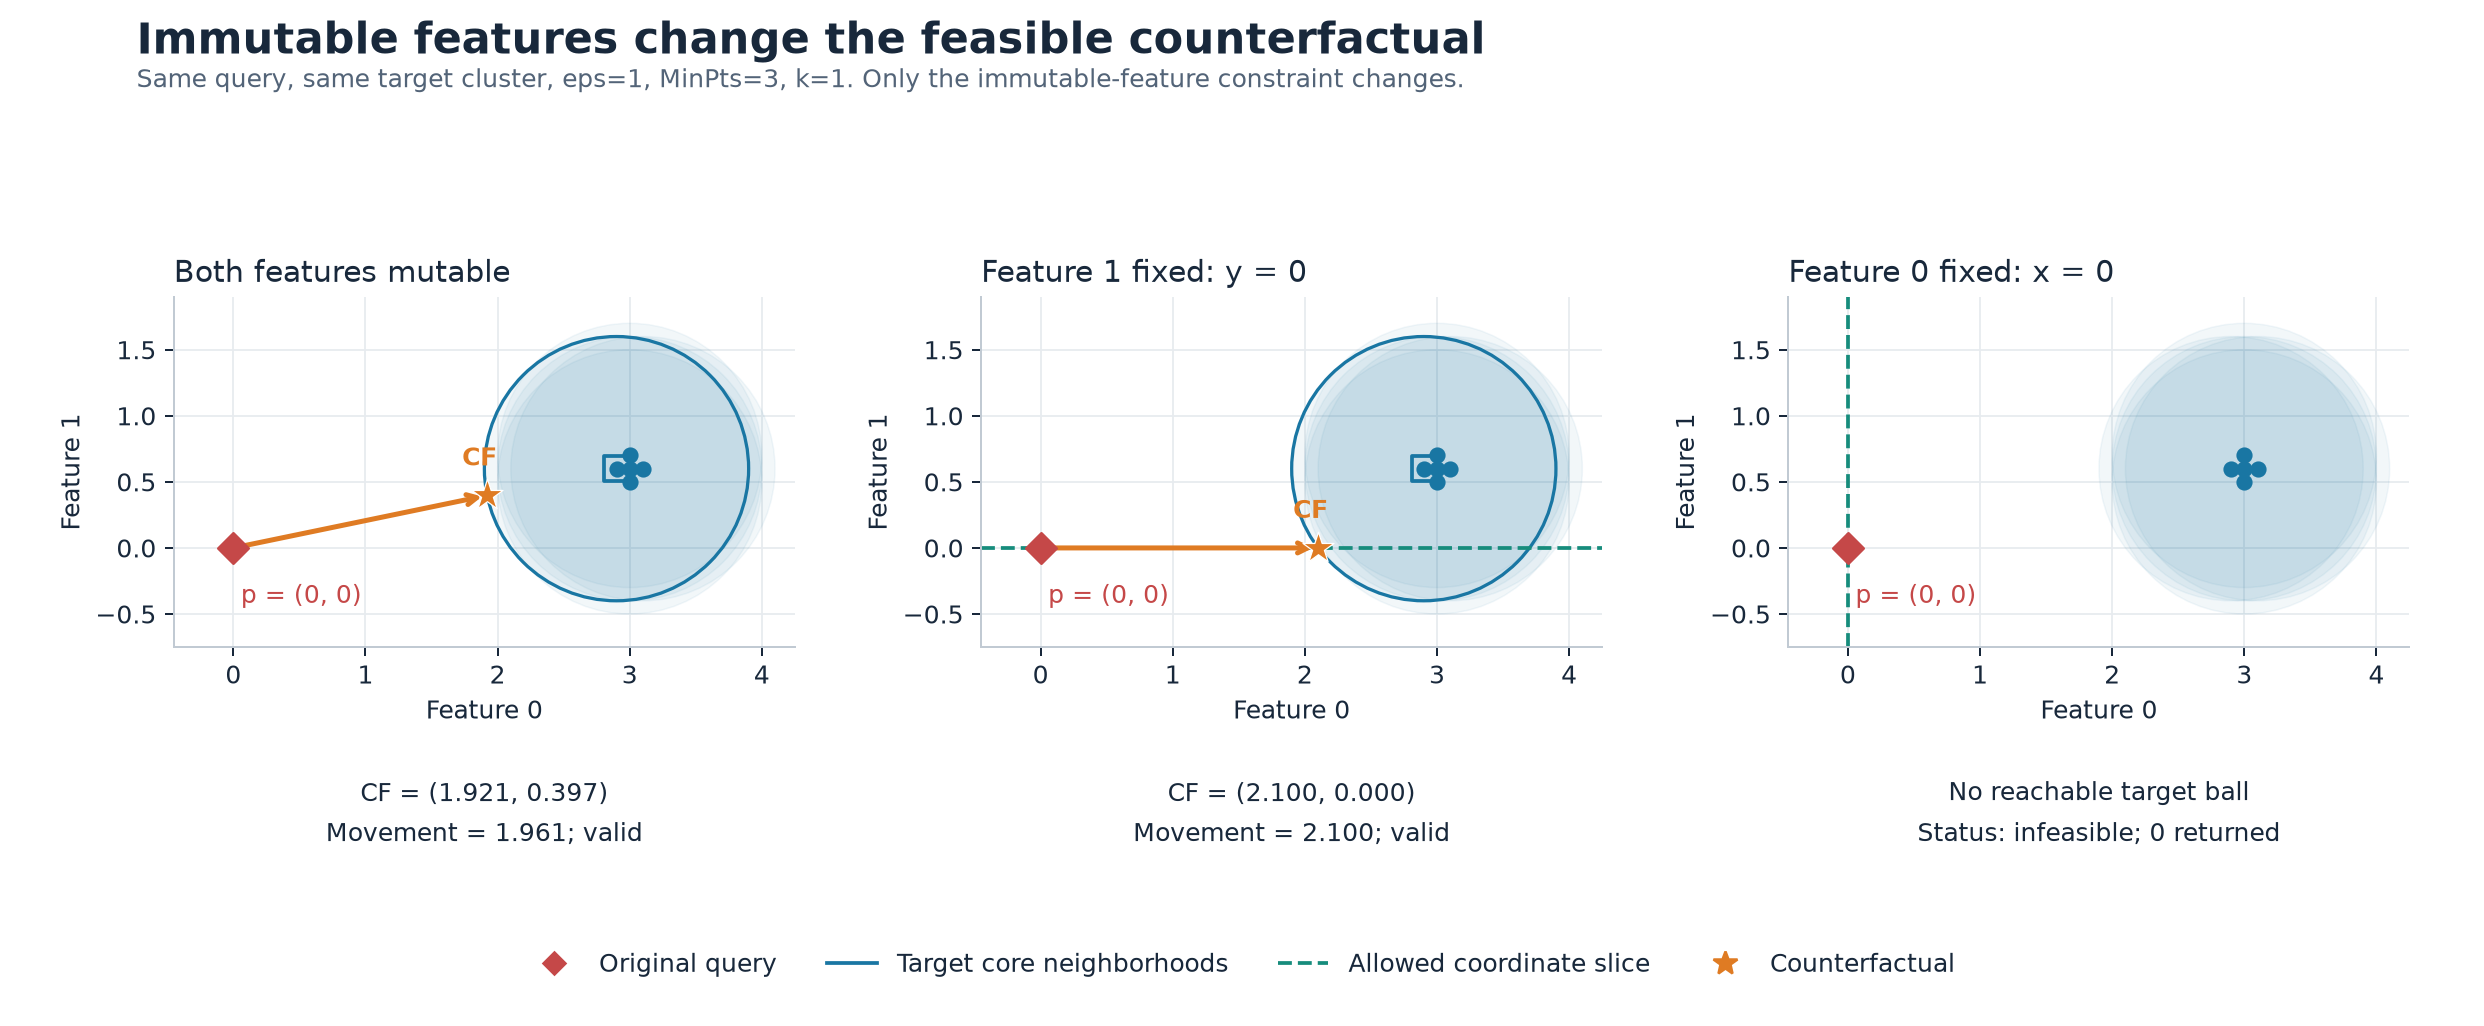
\includegraphics[width=\linewidth,height=0.27\textheight,keepaspectratio]{images/03_constraints.png}
\caption{Effect of fixed coordinates on a synthetic query. The fixed-$y$ case is reachable; fixing $x$ makes the target neighborhood unreachable.}
\label{fig:constraints}
\end{figure}

\section{Interactive Visualization}
The ExDBSCAN Explorer connects a browser interface to the same DBSCAN and ExDBSCAN implementation used in the experiments. A Python service loads the data, fits the model and returns point roles and explanations to a MapLibre-based interface. The Explorer supports the earthquake data and the three synthetic datasets. In the data view, event locations are displayed on a map. In the cluster view (Figure~\ref{fig:explorer-cluster}), sliders change $\eps$ and MinPts, and markers distinguish core points, border points and noise. Selecting an observation, or placing an imagined point, opens its local explanation.

The explanation view combines the selected point's role and neighbor count with a displayed $\eps$-neighborhood and a counterfactual for a chosen target cluster (Figure~\ref{fig:explorer-explain}). The interface reports the size and direction of the change. Direction controls fix either the east--west or north--south coordinate, and the system reports when the target is out of reach. It presents one alternative at a time ($k=1$). A separate check replaces or adds the point and refits DBSCAN, reporting whether it joins the reference point's cluster and whether other point roles change.

\begin{figure}[!htb]
\centering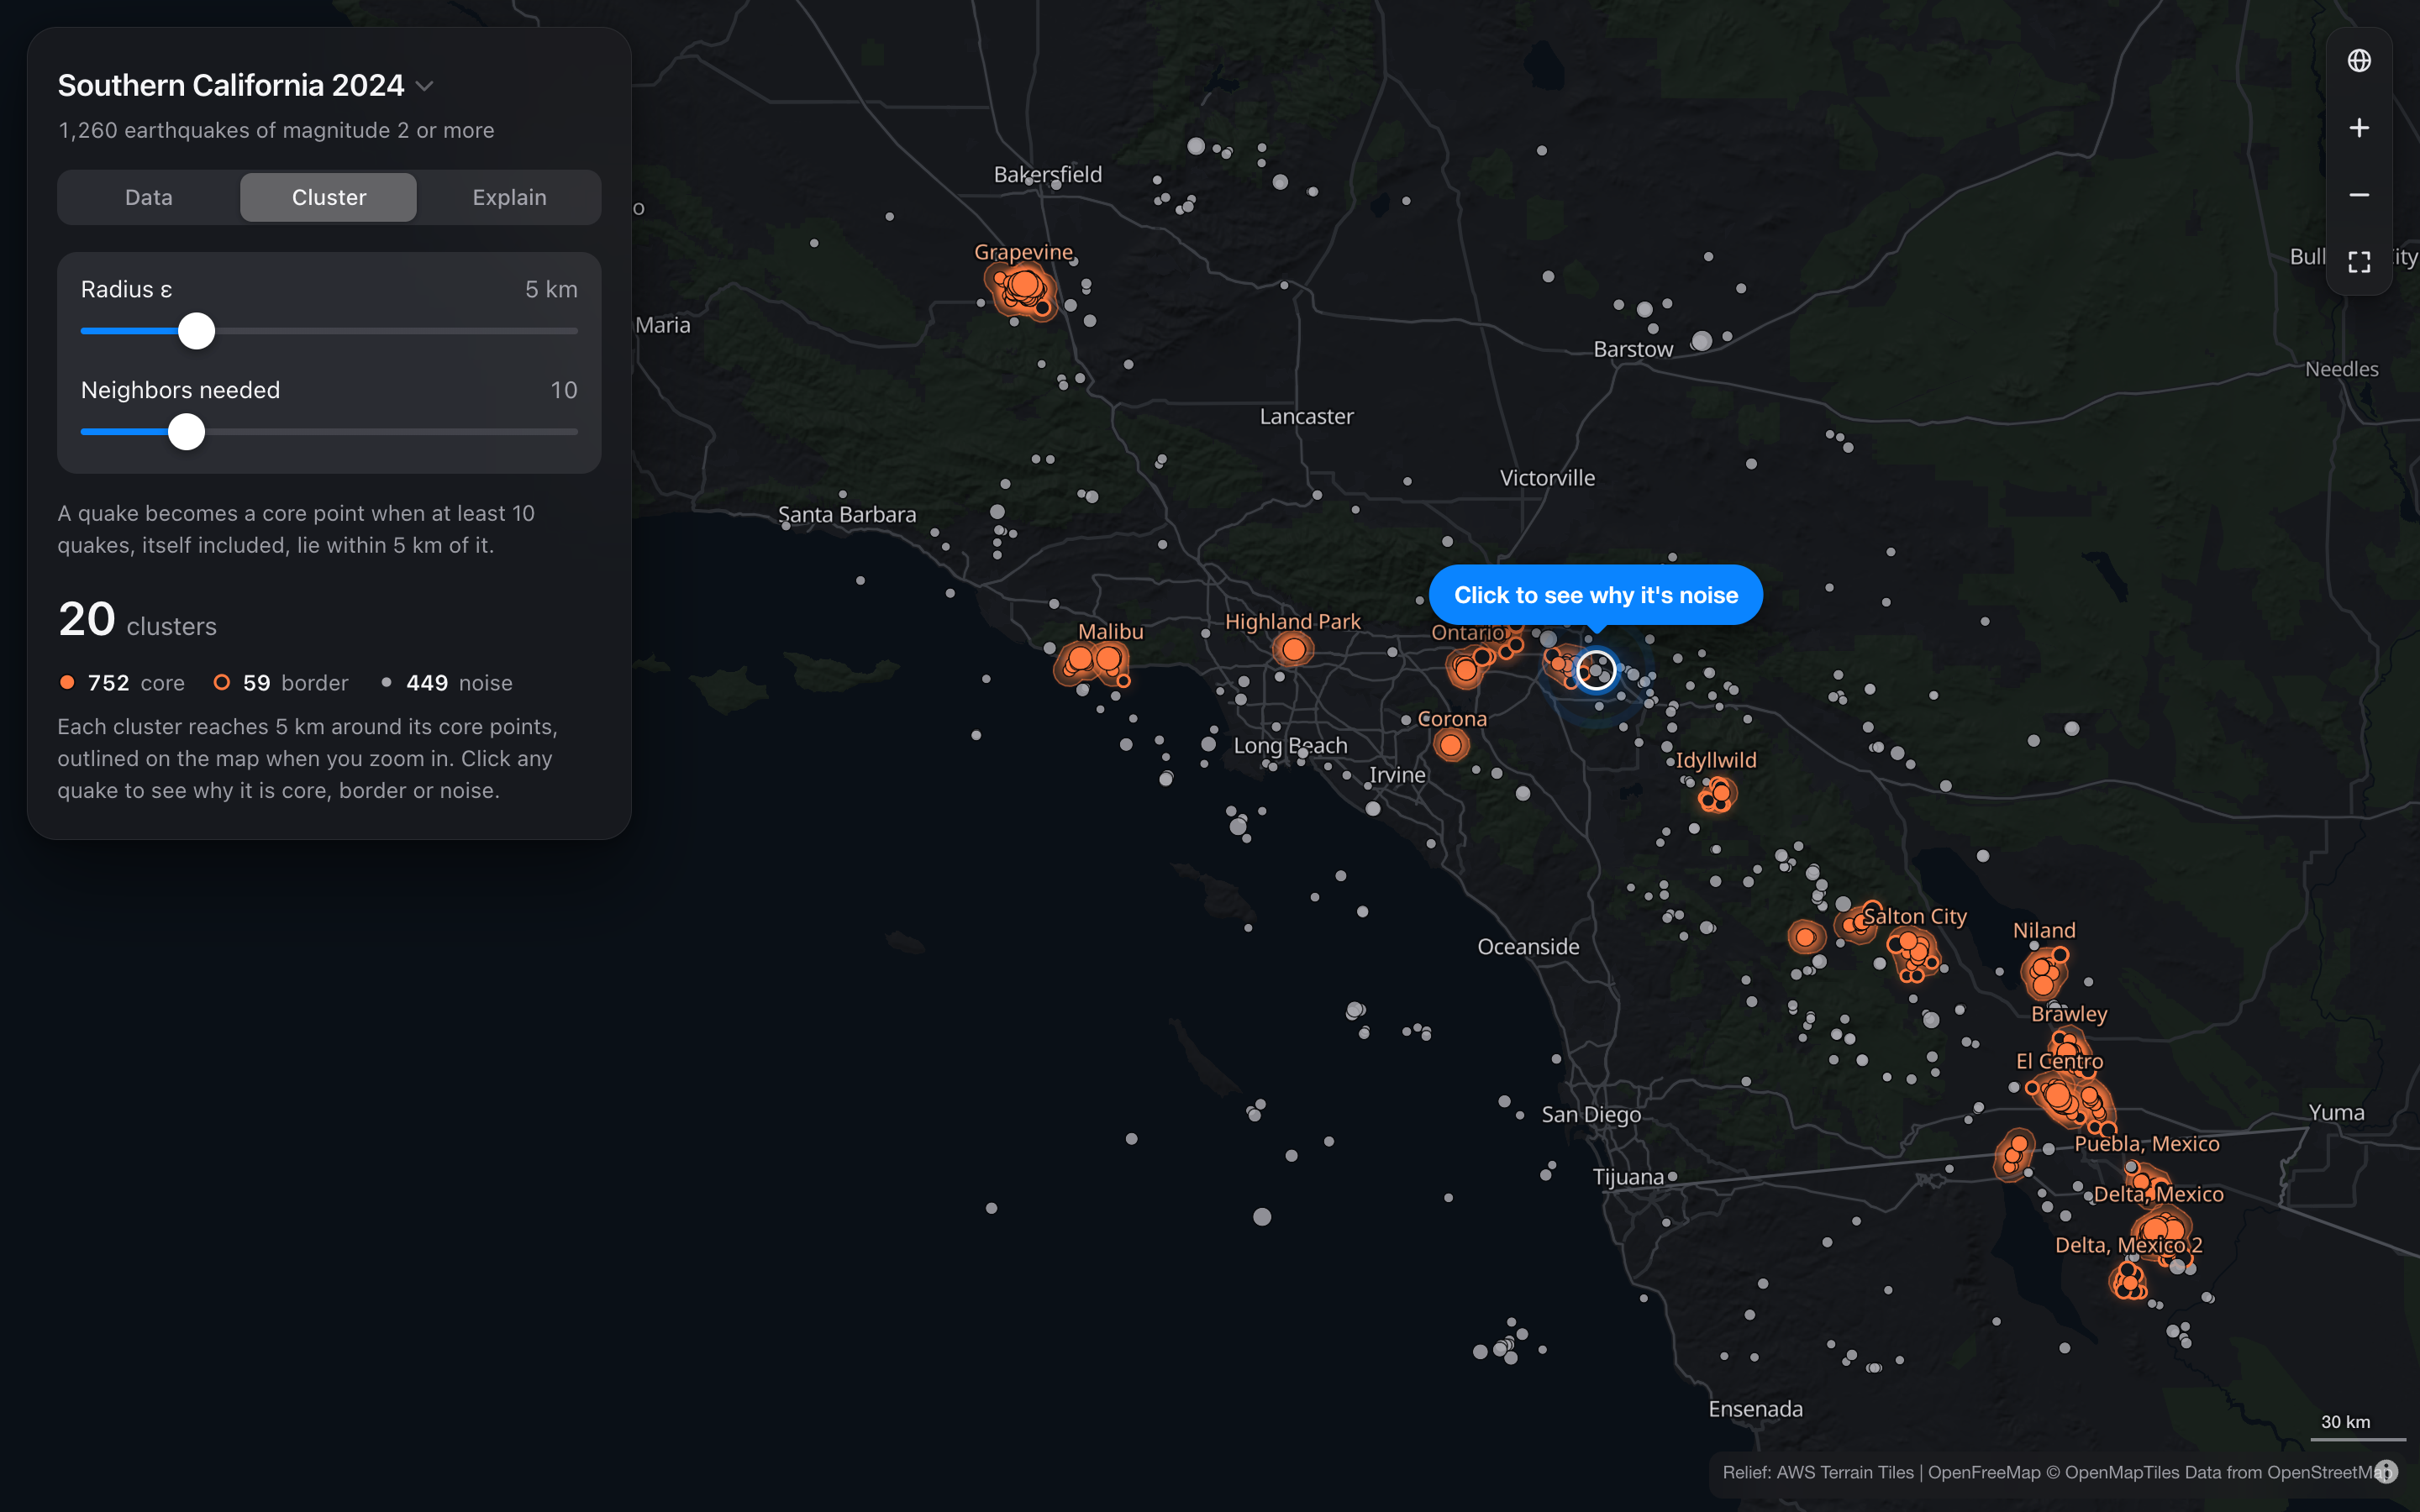
\includegraphics[width=\linewidth,height=0.30\textheight,keepaspectratio]{images/explorer_cluster.png}
\caption{Explorer cluster view for the USGS snapshot at $\eps=5$ km and MinPts $=10$. The panel shows the parameters and point-role counts. Map data: OpenStreetMap contributors; tiles: OpenFreeMap and OpenMapTiles; relief: AWS Terrain Tiles.}
\label{fig:explorer-cluster}
\end{figure}
\FloatBarrier

At the default settings, the model finds 20 clusters: 752 core, 59 border and 449 noise events. In the illustrated case, a magnitude 4.2 event on 25 January 2024 has three events in its neighborhood, including itself, and no core neighbor. The nearest core point is about 8.3 km away. An unconstrained change of about 3.3 km reaches the Loma Linda core neighborhood; the separate refit check places the point in that cluster as a border point. Restricting the change to north--south gives about 3.8 km; restricting it to east--west yields no feasible alternative for that target. These spatial changes are hypothetical feature-space comparisons, not suggested interventions. The views support inspection of the example, but no formal user study was conducted.

\begin{figure}[!htb]
\centering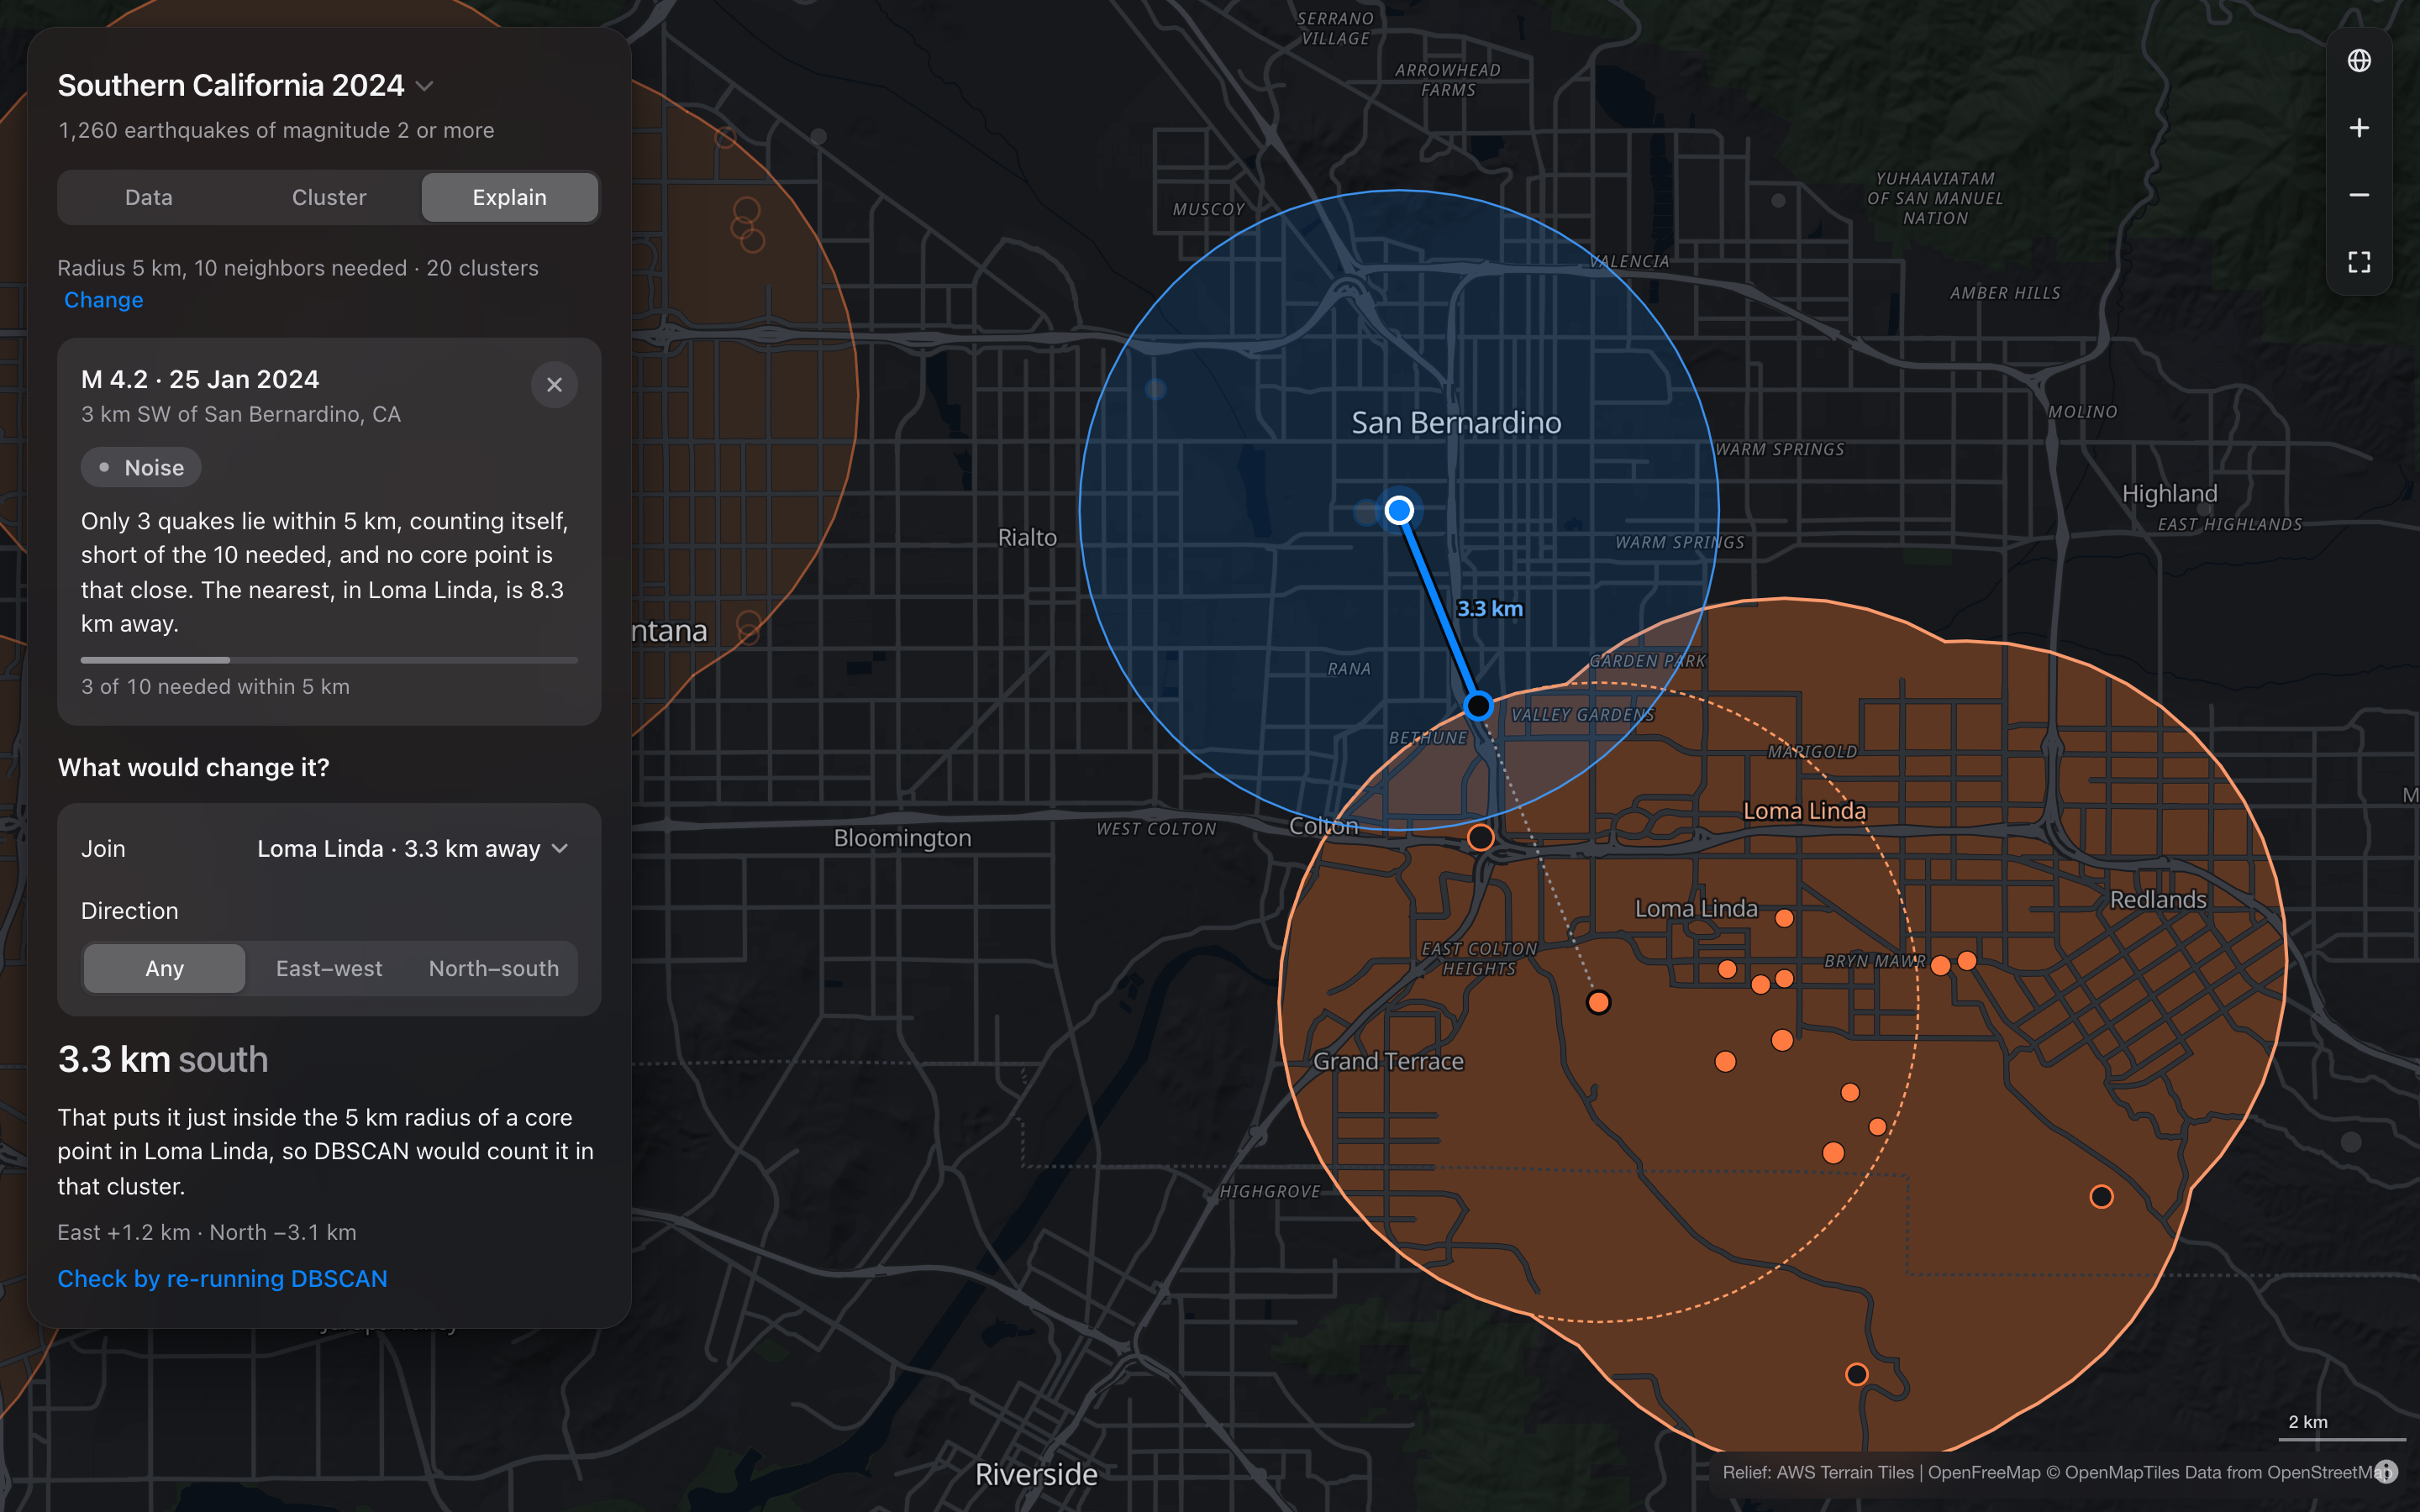
\includegraphics[width=\linewidth,height=0.30\textheight,keepaspectratio]{images/explorer_explain.png}
\caption{Explorer explanation for a noise event near San Bernardino. The blue circle is the query neighborhood; the arrow connects the original point with its counterfactual. The orange region depicts target core neighborhoods. Map data and tiles are attributed as in Figure~\ref{fig:explorer-cluster}.}
\label{fig:explorer-explain}
\end{figure}

\section{Experimental Setup}
\subsection{Datasets and parameters}
We use three controlled two-dimensional datasets: compact blobs with noise, two moons, and concentric rings. These cases expose compact and curved clusters and allow specific point roles to be checked. The saved mock experiments use seeds 7 and 19 and dataset-specific combinations of $\eps$ and MinPts.

The real dataset is a USGS earthquake catalog snapshot \cite{usgs} covering Southern California in 2024 with magnitude at least 2. The recorded snapshot contains 1,260 events. Latitude and longitude are converted to local east and north coordinates in meters using an equirectangular approximation centered at $(34^\circ\mathrm{N},118^\circ\mathrm{W})$. Distances are Euclidean in this projected space, not exact geodesic distances.

The saved real-data grid uses $\eps\in\{2,5,10\}$ km and MinPts $\in\{5,10,20\}$. Both real and synthetic experiments request $k\in\{1,3,5\}$ alternatives and compare greedy, nearest-core, and seeded random reference selection. For each fitted model, the experiment samples up to 12 query--target pairs. Runs are repeated with no fixed feature and with the second coordinate fixed. These repeated configurations are experimental runs, rather than independent real-world events.

\subsection{Validation measures}
Tests cover neighborhood roles, cluster expansion, graph distances, greedy selection, projection, constraints, and data preparation. Graph distances are compared with Floyd--Warshall on test cases, while generated endpoints are checked against target core neighborhoods independently of the selection procedure. The saved validation report records 52 passing unit and property tests.

We distinguish three measures. \emph{Returned validity} is the proportion of returned alternatives that pass the endpoint check. \emph{Requested coverage} is the number of valid alternatives divided by the number requested. \emph{Complete-query rate} is the proportion of requests for which all $k$ requested alternatives are returned and valid. An empty result contributes no valid alternatives to coverage; its returned validity cannot be interpreted as evidence of a valid explanation.

\section{Results and Discussion}
\subsection{Clustering and local explanations}
Figure~\ref{fig:clusters} illustrates DBSCAN on the three synthetic shapes. At the displayed settings, the algorithm identifies compact blobs, curved moons, and concentric rings without being given the number of clusters. The selected examples illustrate the role of density connectivity; they should be interpreted with their specified parameters rather than as a guarantee for every setting.
\begin{figure}[htbp]
\centering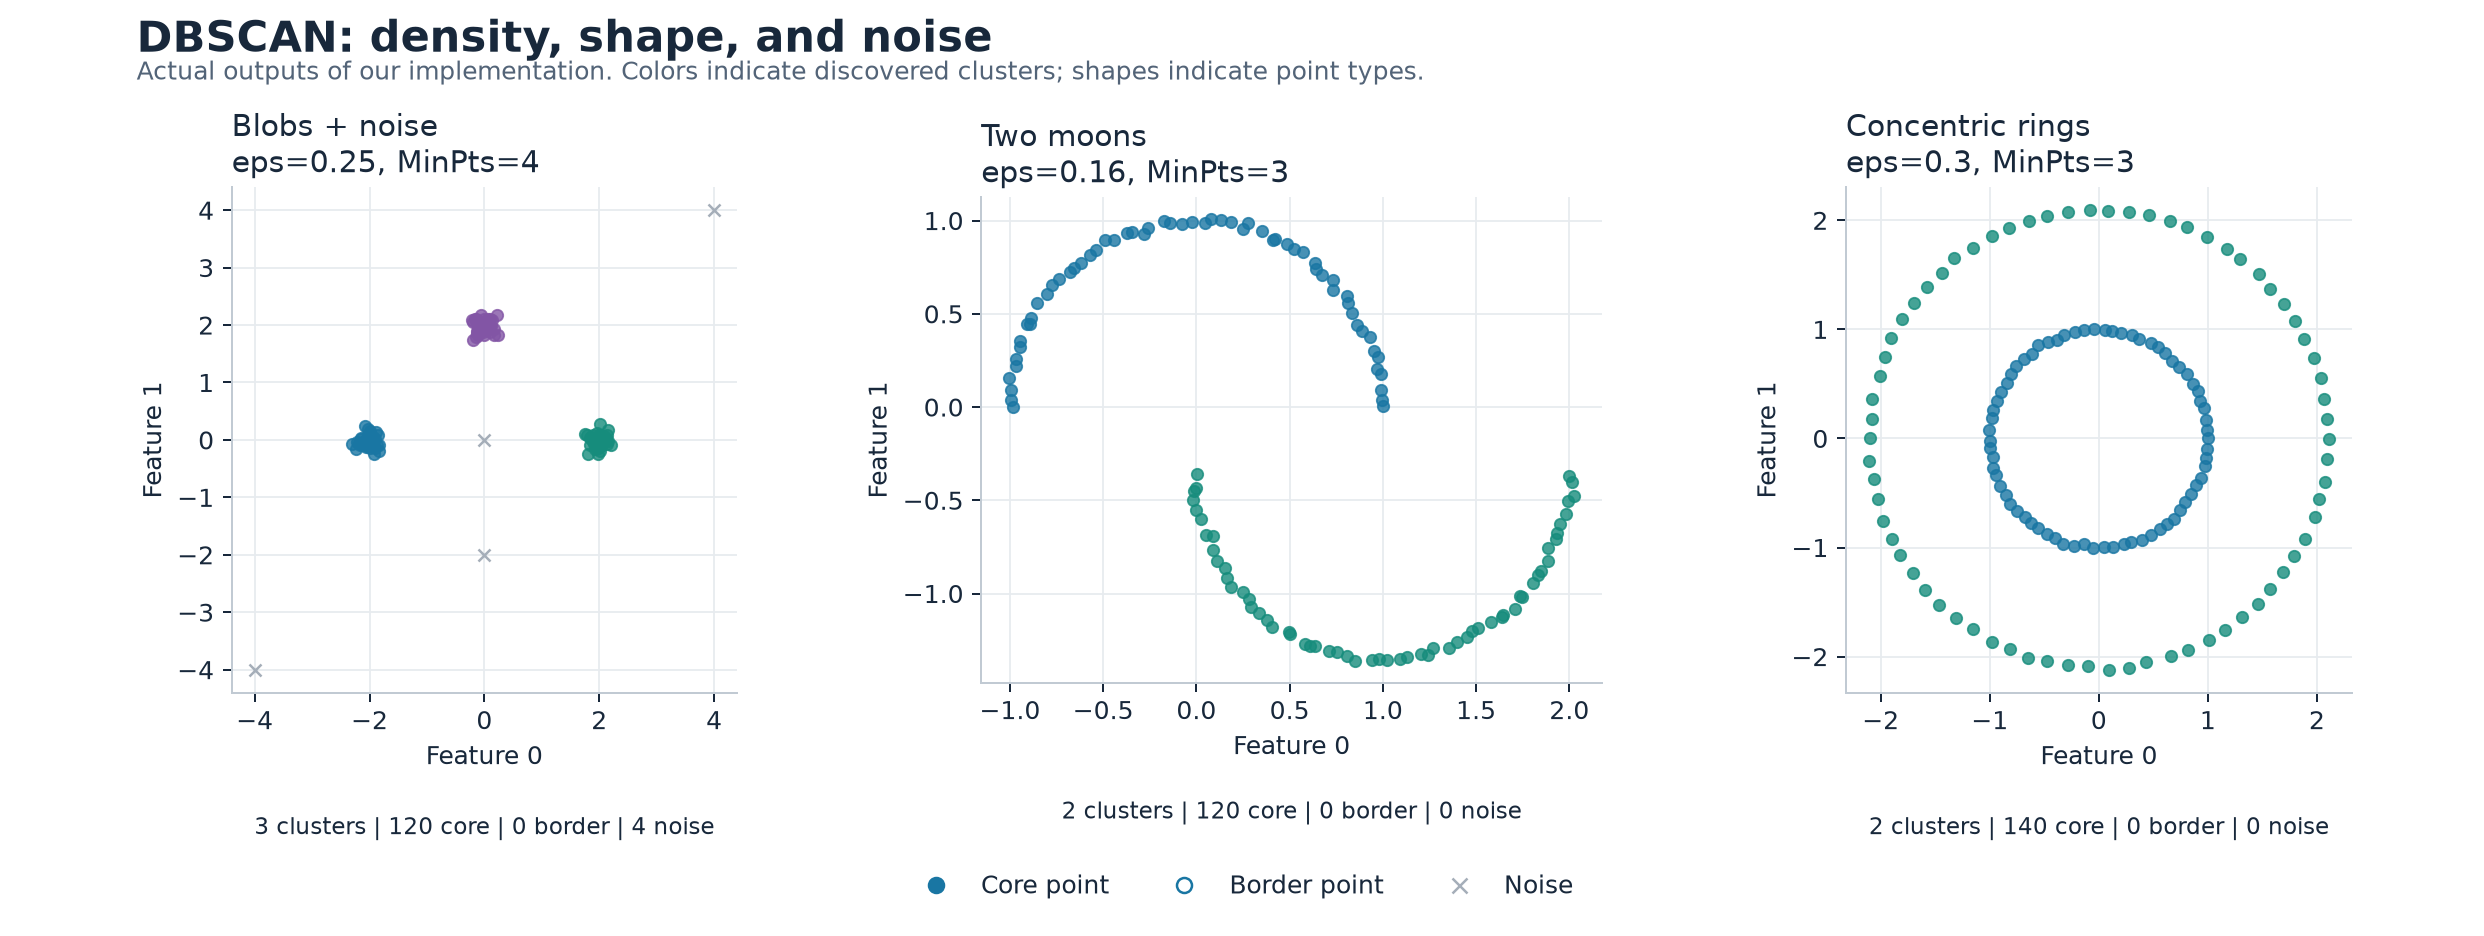
\includegraphics[width=\linewidth,height=0.29\textheight,keepaspectratio]{images/01_dbscan.png}
\caption{DBSCAN results on synthetic blobs, two moons, and rings at representative parameter settings. Filled markers are core points and crosses indicate noise.}
\label{fig:clusters}
\end{figure}

In the local example of Figure~\ref{fig:local}, the role of the selected point follows from the core-point relationship, not only its own neighbor count. Presenting the neighborhood and neighboring core point therefore adds information that is absent from a plain colored scatterplot.

\subsection{Counterfactual validity and coverage}
Across the saved greedy runs, 1,608 query configurations returned 3,184 alternatives, all of which passed the independent target-neighborhood check. This figure excludes the nearest and random strategies. Table~\ref{tab:coverage} separates valid returned points from the proportion of requested points obtained. Unconstrained runs in this sample achieved full requested coverage. With the second coordinate fixed, coverage varies substantially across datasets.
\begin{table}[htbp]
\centering\small
\caption{Greedy results with the second coordinate fixed. Coverage counts valid returned points over requested points; completion counts requests with all requested points valid.}
\label{tab:coverage}
\begin{tabular}{lrrrr}
\toprule
Dataset & Queries & Valid returned & Coverage & Complete \\
\midrule
Blobs & 288 & 432 & 50.00\% & 50.00\% \\
Two moons & 96 & 0 & 0.00\% & 0.00\% \\
Rings & 96 & 234 & 81.25\% & 79.17\% \\
USGS & 324 & 106 & 10.91\% & 10.19\% \\
\bottomrule
\end{tabular}
\end{table}

For the sampled fixed-coordinate moon queries, no requested target neighborhood was reachable. This describes the sampled queries and settings, not every possible constrained moon dataset. Rings and USGS include partial results, so requested coverage and complete-query rate differ. The results show why a high validity rate among returned points should be read together with feasibility and coverage.

\subsection{Proximity and diversity comparison}
Table~\ref{tab:baseline} compares the saved unconstrained two-moons results for $k=3$ using the same 32 query configurations for each strategy. For each query, proximity is the mean distance from the original point to the returned alternatives; the table averages this quantity over queries. Endpoint diversity is the determinant of $K$ with $K_{ij}=1/(1+\|p'_i-p'_j\|)$, averaged over queries. Larger values indicate greater separation under this particular kernel and scale.

\begin{table}[htbp]
\centering\small
\caption{Two-moons comparison for unconstrained queries with $k=3$. All 96 returned alternatives per strategy passed the target-neighborhood check.}
\label{tab:baseline}
\begin{tabular}{lrr}
\toprule
Reference selection & Mean proximity $\downarrow$ & Endpoint diversity $\uparrow$ \\
\midrule
Greedy & 0.972 & 0.232 \\
Nearest & 0.893 & 0.033 \\
Random & 1.572 & 0.304 \\
\bottomrule
\end{tabular}
\end{table}

Nearest selection gives the smallest mean change in this sample but the lowest measured diversity. Random selection gives the highest diversity and the largest mean change; greedy lies between them on both measures. The comparison illustrates a proximity--diversity trade-off for these settings, not a general ranking. Diversity depends on the feature scale and kernel, so these values should not be compared directly with the spatial dataset or other studies.

\subsection{Spatial example and parameter sensitivity}
At $\eps=2$ km and MinPts $=5$, DBSCAN finds 30 clusters in the USGS snapshot. Figure~\ref{fig:real} shows an overview and a target-cluster explanation. The selected target is cluster 0, which need not be the nearest alternative; the displayed movement should not be read as the minimum distance to any cluster. Figure~\ref{fig:validation} summarizes the separate coverage measures.
\begin{figure}[htbp]
\centering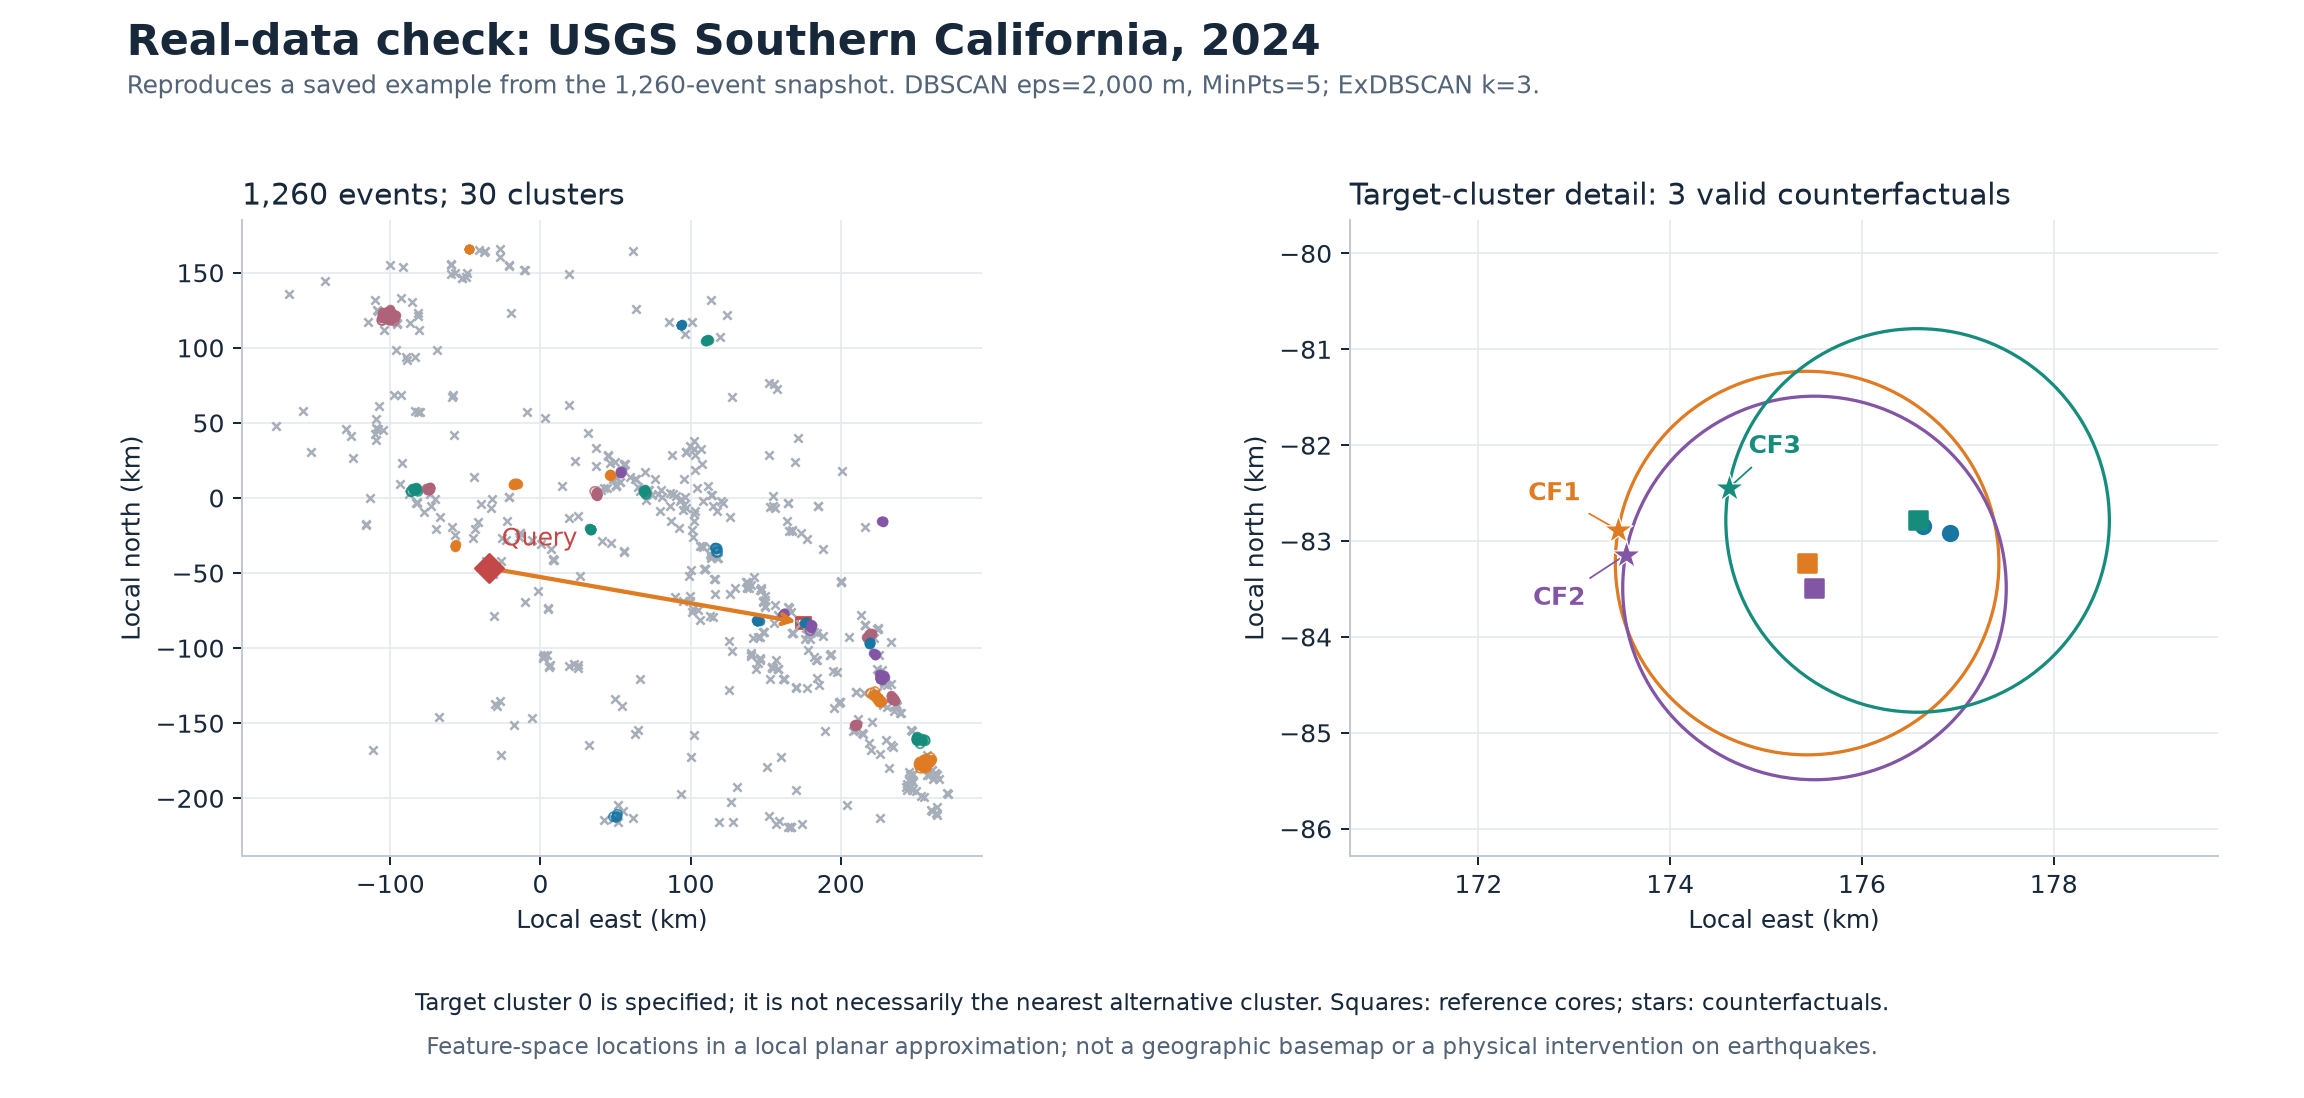
\includegraphics[width=\linewidth,height=0.29\textheight,keepaspectratio]{images/05_real_data.png}
\caption{USGS snapshot: clustering overview and an enlarged target-cluster example. Coordinates are projected spatial features; the alternative positions are hypothetical.}
\label{fig:real}
\end{figure}
\begin{figure}[htbp]
\centering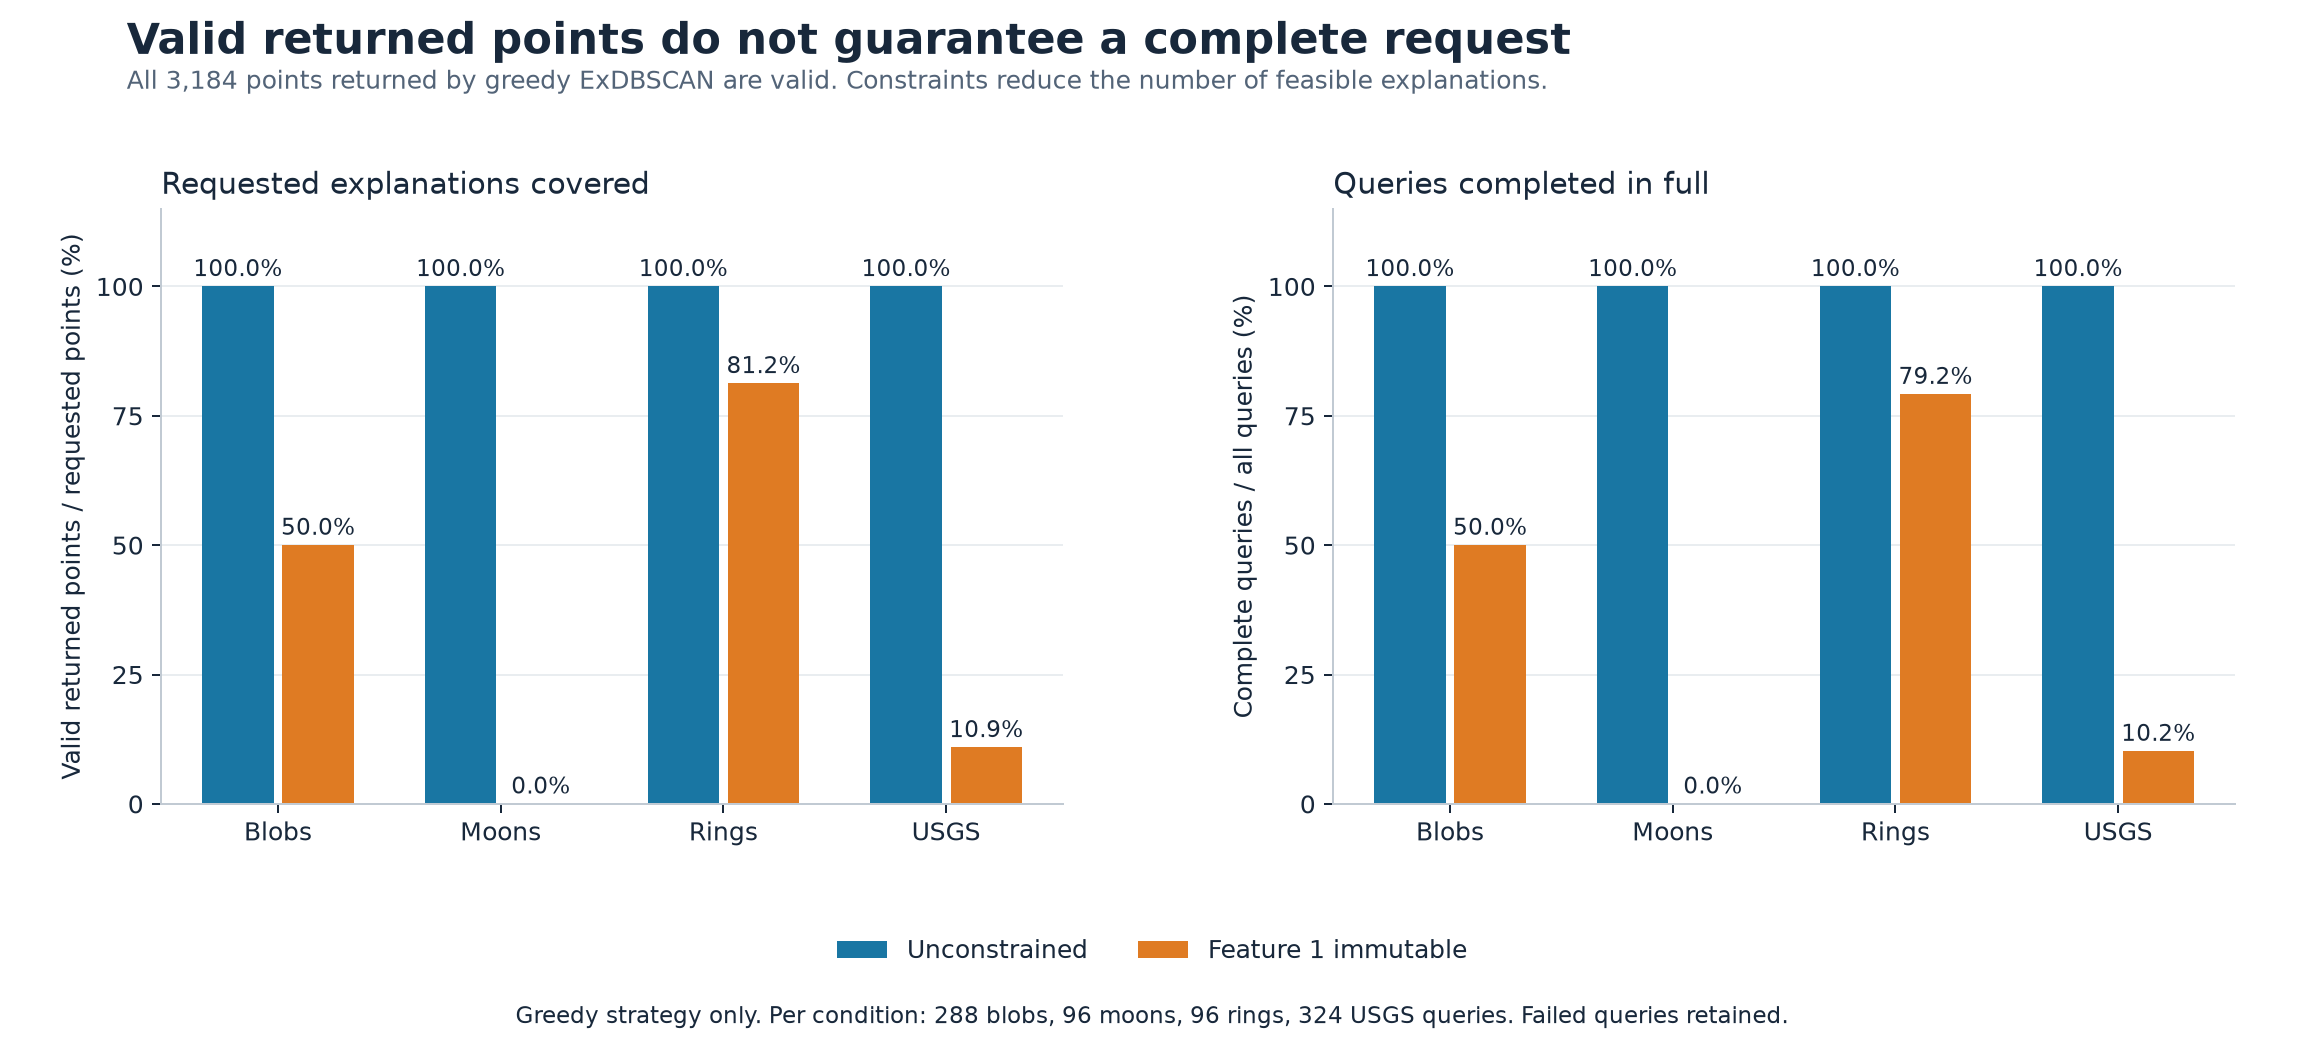
\includegraphics[width=\linewidth,height=0.25\textheight,keepaspectratio]{images/04_validation.png}
\caption{Requested coverage and complete-query rates for greedy explanations. The constrained runs retain partial and infeasible cases.}
\label{fig:validation}
\end{figure}

The parameter sweep in the visual results uses 56 combinations of $\eps$ and MinPts on the same 1,260 events. At MinPts $=5$, the number of clusters rises from 26 to 37 and then falls to 12 across the tested radii as neighborhoods and clusters merge. Across the grid, the noise fraction ranges from 2.7\% to 79.4\%. The result emphasizes that both a point's role and its counterfactual explanation depend on the fitted clustering. A visual explanation should therefore show the parameter setting alongside the result.

\section{Conclusion and Limitations}
The project links density-based clustering to local and counterfactual views. Controlled examples explain point roles and graph-based alternatives; the USGS example illustrates the same ideas on spatial observations. The experiments show valid returned alternatives under the stated fixed-clustering check, while fixed features can make requests partially or completely infeasible.

Interpretation remains dependent on $\eps$, MinPts, the distance measure, and the sampled dataset. The current implementation uses Euclidean numeric features and is intended for small-scale experiments; it does not establish large-scale performance. A target-neighborhood check and a fresh DBSCAN fit answer different questions. Future work could investigate additional datasets and feature constraints, controlled performance measurements, and a user study of the visual explanations.

\FloatBarrier
\bibliographystyle{unsrt}
\bibliography{references}

\section*{Group Members}
\enlargethispage{2\baselineskip}
\textbf{Group 1} \quad | \quad \textbf{Project type:} Implementation

Although the project includes visualization, it studies density-based clustering and counterfactual explanations rather than the members' topics in human--computer interaction research, video--audio or long-video generation, multimodal language models, or language-agent policy compliance.

\small
\begin{tabularx}{\linewidth}{@{}l l l X@{}}
\toprule
Name & Student ID & Supervisor & Research topic \\
\midrule
Jianheng Ouyang & 21197820 & Arpit Narechania & Human--computer interaction \\
Pengjun Fang & 20944434 & Qifeng Chen & Video--audio joint generation \\
Yifei Jia & 20934910 & Qifeng Chen & Long video generation \\
Shangpin Peng & 21324576 & Jiaya Jia & Multimodal large language models \\
Wu Kam Man & 20922773 & Qifeng Chen & Video--audio joint generation \\
Sirui Zhang & 21403231 & Yangqiu Song & Policy compliance in language-model agents \\
\bottomrule
\end{tabularx}
\normalsize

\noindent\textbf{Course declaration.} As stated in the group proposal, each member declares that this project is conducted solely within COMP5331 and is not submitted or developed as part of another course, research project, or FYP.

\makeatletter
\renewcommand{\subsection}{\@startsection{subsection}{2}{\z@}{0.6ex}{0.35ex}{\normalfont\normalsize\bfseries}}
\makeatother
\setlength{\parskip}{2pt}
\section*{Contribution}
\subsection*{Jianheng Ouyang}
I worked on the data and DBSCAN components of the project. I examined the synthetic datasets and USGS earthquake data used in our experiments, focusing on their spatial features and how DBSCAN identifies core, border, and noise points. I developed an illustrative example showing a point's neighborhood and explaining why it is classified as a border point. I updated the corresponding figure, documentation, and visual-results report, and verified that the example could be reproduced using the existing tests. In addition, I wrote the final project paper, covering the implementation, experimental results, visual explanations, and their connections to the course.
\subsection*{Pengjun Fang}
\todo{Contribution to be added.}

\subsection*{Yifei Jia}
\todo{Contribution to be added.}

\subsection*{Shangpin Peng}
\todo{Contribution to be added.}

\newpage
\subsection*{Wu Kam Man}
I worked on stabilizing the existing ExDBSCAN implementation by adding certified positional robustness and parameter-stability evaluation. For a requested tolerance, I implemented projection onto shrunken neighborhoods of target core points and selected the feasible endpoint with the smallest movement, while preserving immutable coordinates. I derived the certificate using the triangle inequality and documented that it applies to reachability in a fixed clustering snapshot. I also implemented a parameter-grid check that refits DBSCAN and matches clusters through membership overlap, explicitly reporting splits, merges, and disappearance. I evaluated the extension on synthetic datasets and the USGS earthquake snapshot, comparing it with the original method and a simple inward-movement baseline. I added regression tests, reproducible experiment outputs, and an interactive comparison page showing movement costs, error circles, and stability grids. I also unified numerical tolerances so floating-point boundary errors would not exaggerate the measured improvement.

\subsection*{Sirui Zhang}
I worked on the interactive visualization part of the project and built the ExDBSCAN Explorer. I wrote a small Python server that loads the earthquake and synthetic datasets and calls the group's DBSCAN and ExDBSCAN implementation, so the Explorer shows the same results as our experiments. I built the map interface with MapLibre and drew each event through the exact inverse of the projection used in our experiments, so that every $\eps$-neighborhood on the map is the one DBSCAN uses. In the interface, a user can change $\eps$ and MinPts, see why a point is a core point, a border point or noise, and find the smallest move that puts it into a chosen cluster, with the option of fixing one coordinate. I also added the check that moves the point and fits DBSCAN again. Because a counterfactual lies exactly on the $\eps$ boundary, floating-point rounding could leave it just outside, so the check moves the point a further $10^{-9}$ of the way inside. I wrote the Explorer's documentation and took the screenshots used in Figures~\ref{fig:explorer-cluster} and~\ref{fig:explorer-explain}.

\end{document}
